\documentclass[a4paper]{article}
\usepackage{amsfonts}
\usepackage{amsmath}
\usepackage{amssymb}
\usepackage{graphicx}     

\newcommand{\dint}{\displaystyle\int}
\newcommand{\ldint}{\dint\limits_1^2}

\begin{document}
  
\noindent \large Auteur: Thijs Van Schel \\
\noindent \large Studierichting: Informatica\\
\noindent \large Oefeningenreeks 5G nr. 4.3\\

\medskip

\normalsize

$f(y) = \sqrt(1+y^3)$ op het interval $[1,2]$\\

$\pi\ldint(1+y^3)dy=\pi\ldint dy + \pi\ldint y^3dy$\\

$=\pi\left[y+\dfrac{y^4}{4}\right]_1^2$\\

$= \pi+4\pi-\dfrac{\pi}{4} = \dfrac{19\pi}{4}$\\

Tekening: \\

\begin{figure}[h]
\centering
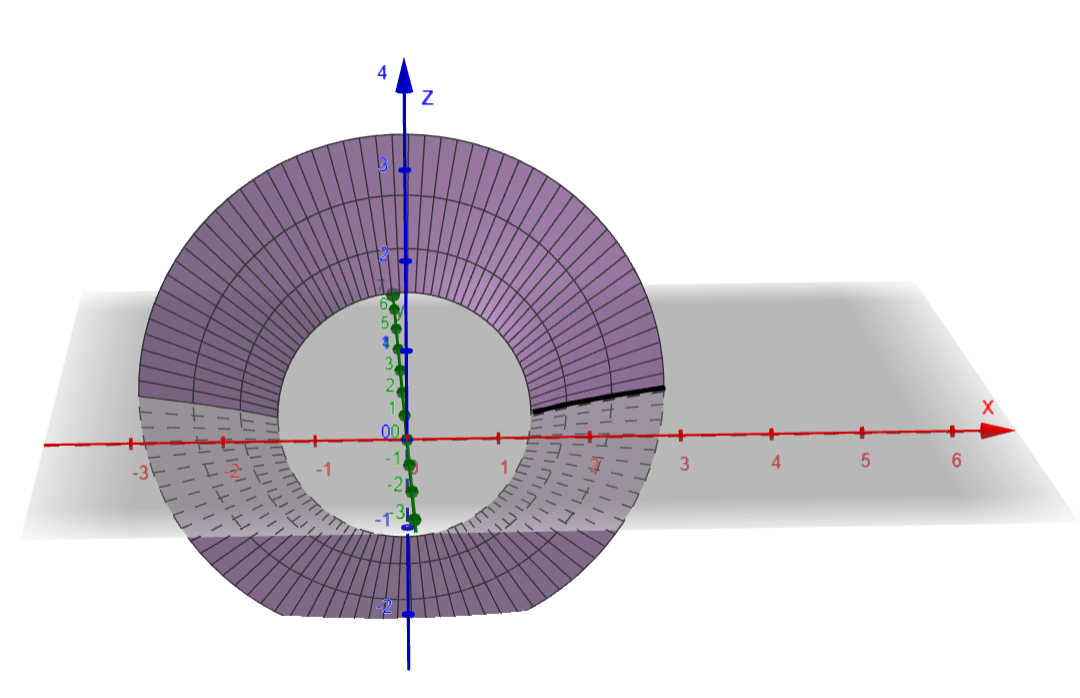
\includegraphics[width=0.5\linewidth]{5G-4.3-thijs.van.schel.INF.png}
\end{figure} 

\begin{thebibliography}{999}
%\bibitem{a} Referentie
\end{thebibliography}
\end{document} 
